\documentclass[light, handout]{presentation}

\pdfauthor{Venkat}
\pdftitle{EMNLP 2020 Presentation}

\usepackage{multirow}
\usepackage{pgf-pie}
\usepackage{subcaption}
\usepackage{tikz}
\usepackage{appendixnumberbeamer}

\graphicspath{{figures/}}
\captionsetup{labelformat=empty}
\addbibresource{references.bib}

% To do overlay stuff in tikz and loading tikz patterns
\usetikzlibrary{patterns}
\tikzset{
    invisible/.style={opacity=0},
    visible on/.style={alt={#1{}{invisible}}},
    alt/.code args={<#1>#2#3}{%
      \alt<#1>{\pgfkeysalso{#2}}{\pgfkeysalso{#3}} % \pgfkeysalso doesn't change the path
    },
  }

% Title stuff
\title{Help! Need Advice on Identifying Advice}
\subtitle{\sansc EMNLP 2020}
\date{}
\author{\small Venkata S Govindarajan$^1$, Benjamin T Chen$^2$,
        Rebecca Warholic$^3$, \\
        Katrin Erk$^1$, Junyi Jessy Li$^1$}
\institute{$^1$ The University of Texas at Austin\\
           $^2$ Amazon Inc.\\
           $^3$ McGill University}


\begin{document}

\maketitle

{
\metroset{sectionpage=none}
\section{Motivation}
\begin{frame}[c]\frametitle{Motivation - Advice Strategies}

\pause

\begin{center}
\vfill \itshape \large Parenting with a history of depression?
\end{center}

\ex. \label{ex:2} \vfill \alert<3->{I took} my meds the whole time. \alert<3->{I used} the tools I learned in therapy. \alert<3->{I talked} on Reddit with others to get support and ideas.

\qquad \qquad \qquad \qquad \qquad \qquad \qquad \qquad \qquad \qquad \qquad \qquad (r/AskParents)

\pause

\vfill People often give advice \textbf{implicitly} using personal narratives and other strategies~\citep{abolfathiasl2013pragmatic}.

\end{frame}


\begin{frame}[c]\frametitle{Motivation - Non Advice}

\pause

\begin{center}
\vfill \itshape \large Is it too late to start a hobby/activity at 12?
\end{center}

\ex. \label{ex:1}  \vfill ..\alert<3->{you can always pick anything up you think is interesting and giving it a shot}. You never know what you are good at until you try new things! \alert<3->{Idk if you have a budget or maybe borrow tools but you can try woodworking?} It’s fun and frustrating (in a good way) at the same time

\qquad \qquad \qquad \qquad \qquad \qquad \qquad \qquad \qquad \qquad \qquad \qquad (r/needadvice)

\pause

\vfill Advice is often \textbf{interspersed} with support, reassurance and reasoning.

\end{frame}


}

{
\metroset{sectionpage=none}
\section{Related Work}
\begin{frame}[c]\frametitle{Related Work}

\begin{center}
\alert{\large How do people give advice (online)?}
\end{center}

\pause

\vfill

\begin{description}[Suggestion Mining]\itemsep10pt
    \item[Advice Questions] Dataset of advice-seeking intentions from personal narratives~\citep{fu-etal-2019-asking}.

    \item[Suggestion Mining] SemEval-2019 introduced a pilot task on suggestion mining but suggestions are not synonymous with advice~\citep{negi-etal-2019-semeval}.

    \item[TuringAdvice] A framework that evaluates language models by asking them to generate useful advice for humans~\citep{zellers2020evaluating}.
\end{description}


\end{frame}


\begin{frame}[c]\frametitle{Our questions}

\pause

\textbf{How is advice structured online?}

This work aims to advance both our understanding of how people give advice, as well as to provide resources for learning to identify advice

\pause

\vspace{5mm}

\textbf{How good are computational models at identifying advice?}

We establish preliminary baselines with rule-based models~\citep{negi-etal-2019-semeval,potamias-etal-2019-ntua} and BERT~\citep{devlin_bert:_2019}, and analyze their performance.

\end{frame}
}

{
\section{Annotation Protocol and Dataset}
\begin{frame}[c]\frametitle{Data Sources}

To model general online human advice-seeking interactions, we chose to construct datasets from Reddit forums (subreddits) focused on advice.

\pause

\vspace{10mm}

\begin{table}[H]
    \centering
    \begin{tabular}{ll}
        \toprule
        \textbf{r/AskParents} & \textbf{r/needadvice} \\ \midrule
        parents seeking advice & a general advice forum \\ \midrule
        less moderation & more moderation\\ \midrule
        \multirow{3}{*}{no flairs} & 5 flairs -- ``Education'', ``Career'',\\
        & ``Mental Health'', ``Life Decisions'', \\
        & ``Friendships''\\ \bottomrule
    \end{tabular}
    \label{tab:datasources}
\end{table}

\end{frame}


\begin{frame}[c]\frametitle{Annotation}
    \begin{figure}
        \centering
        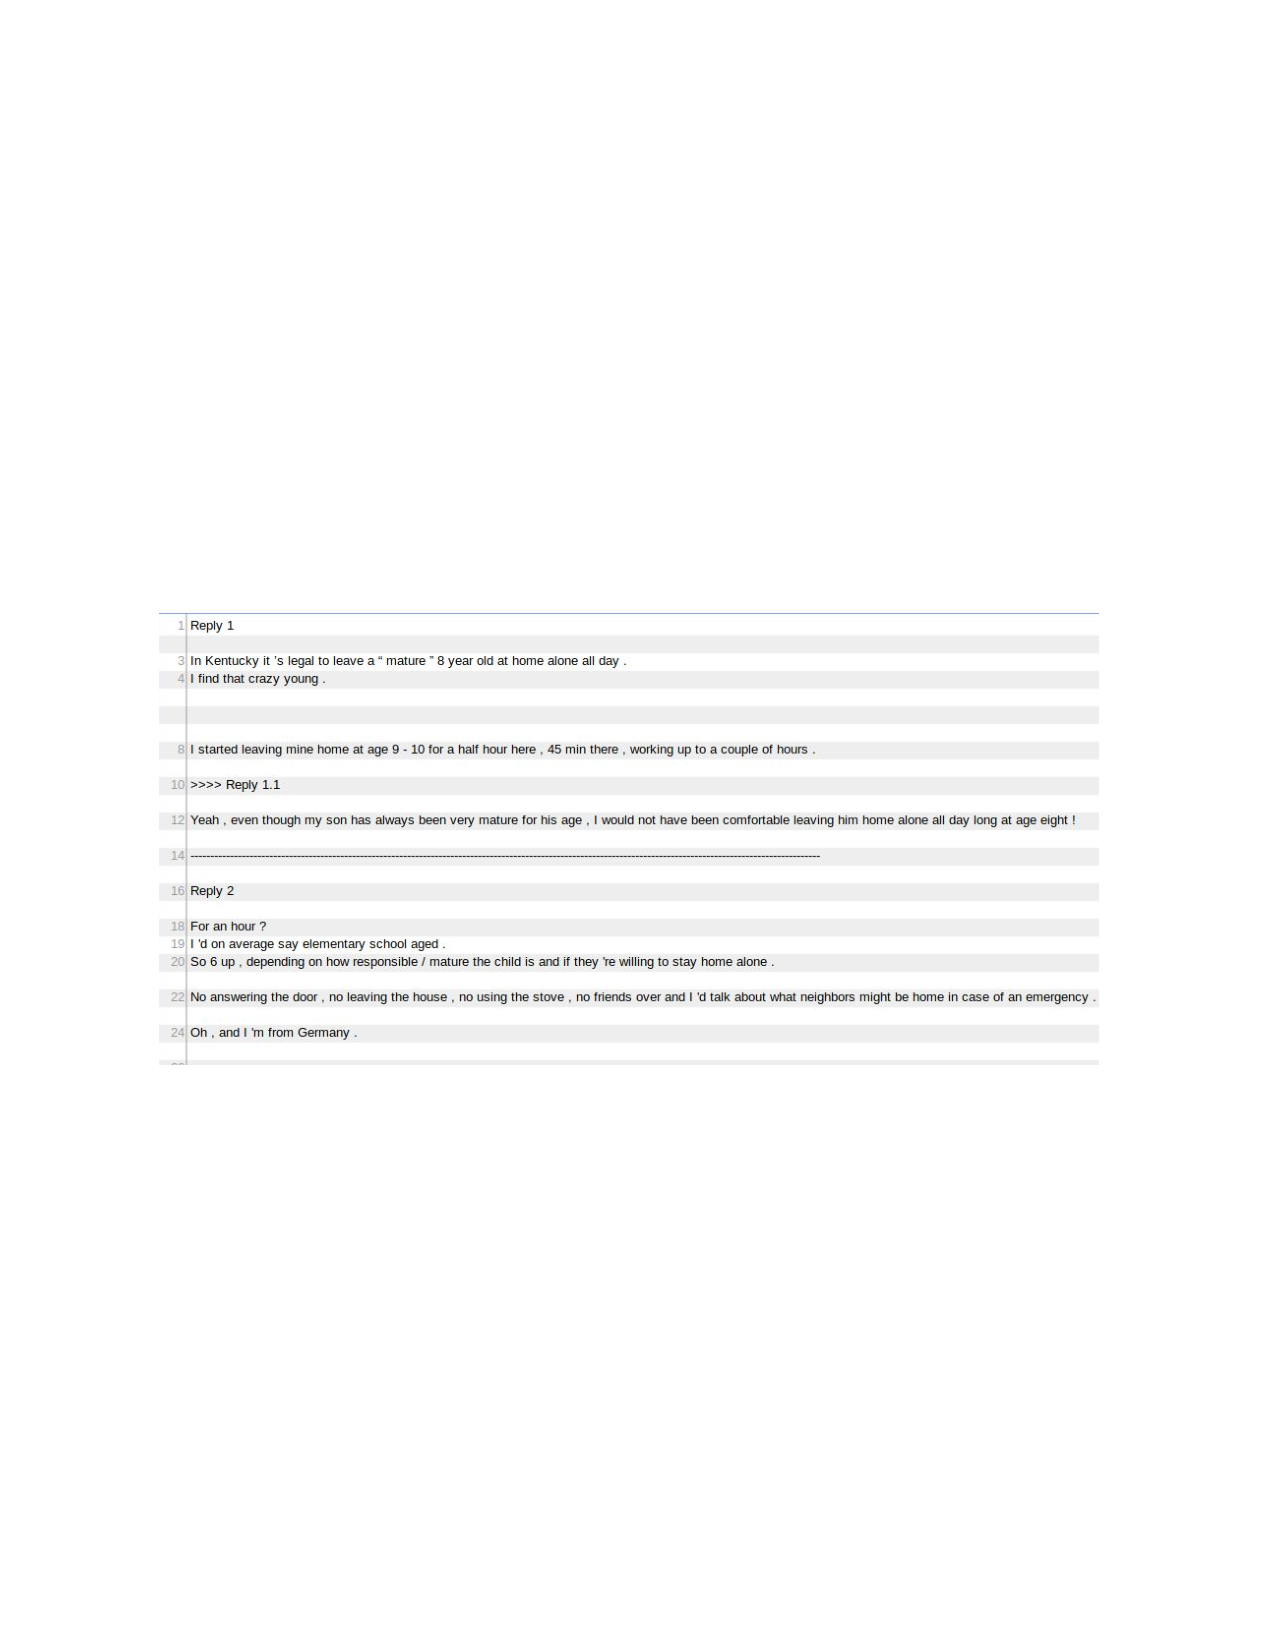
\includegraphics[width=\linewidth]{figures/ann-1.pdf}
        \caption{}
    \end{figure}
\end{frame}

\begin{frame}[c]\frametitle{Annotation}
    \begin{figure}
        \centering
        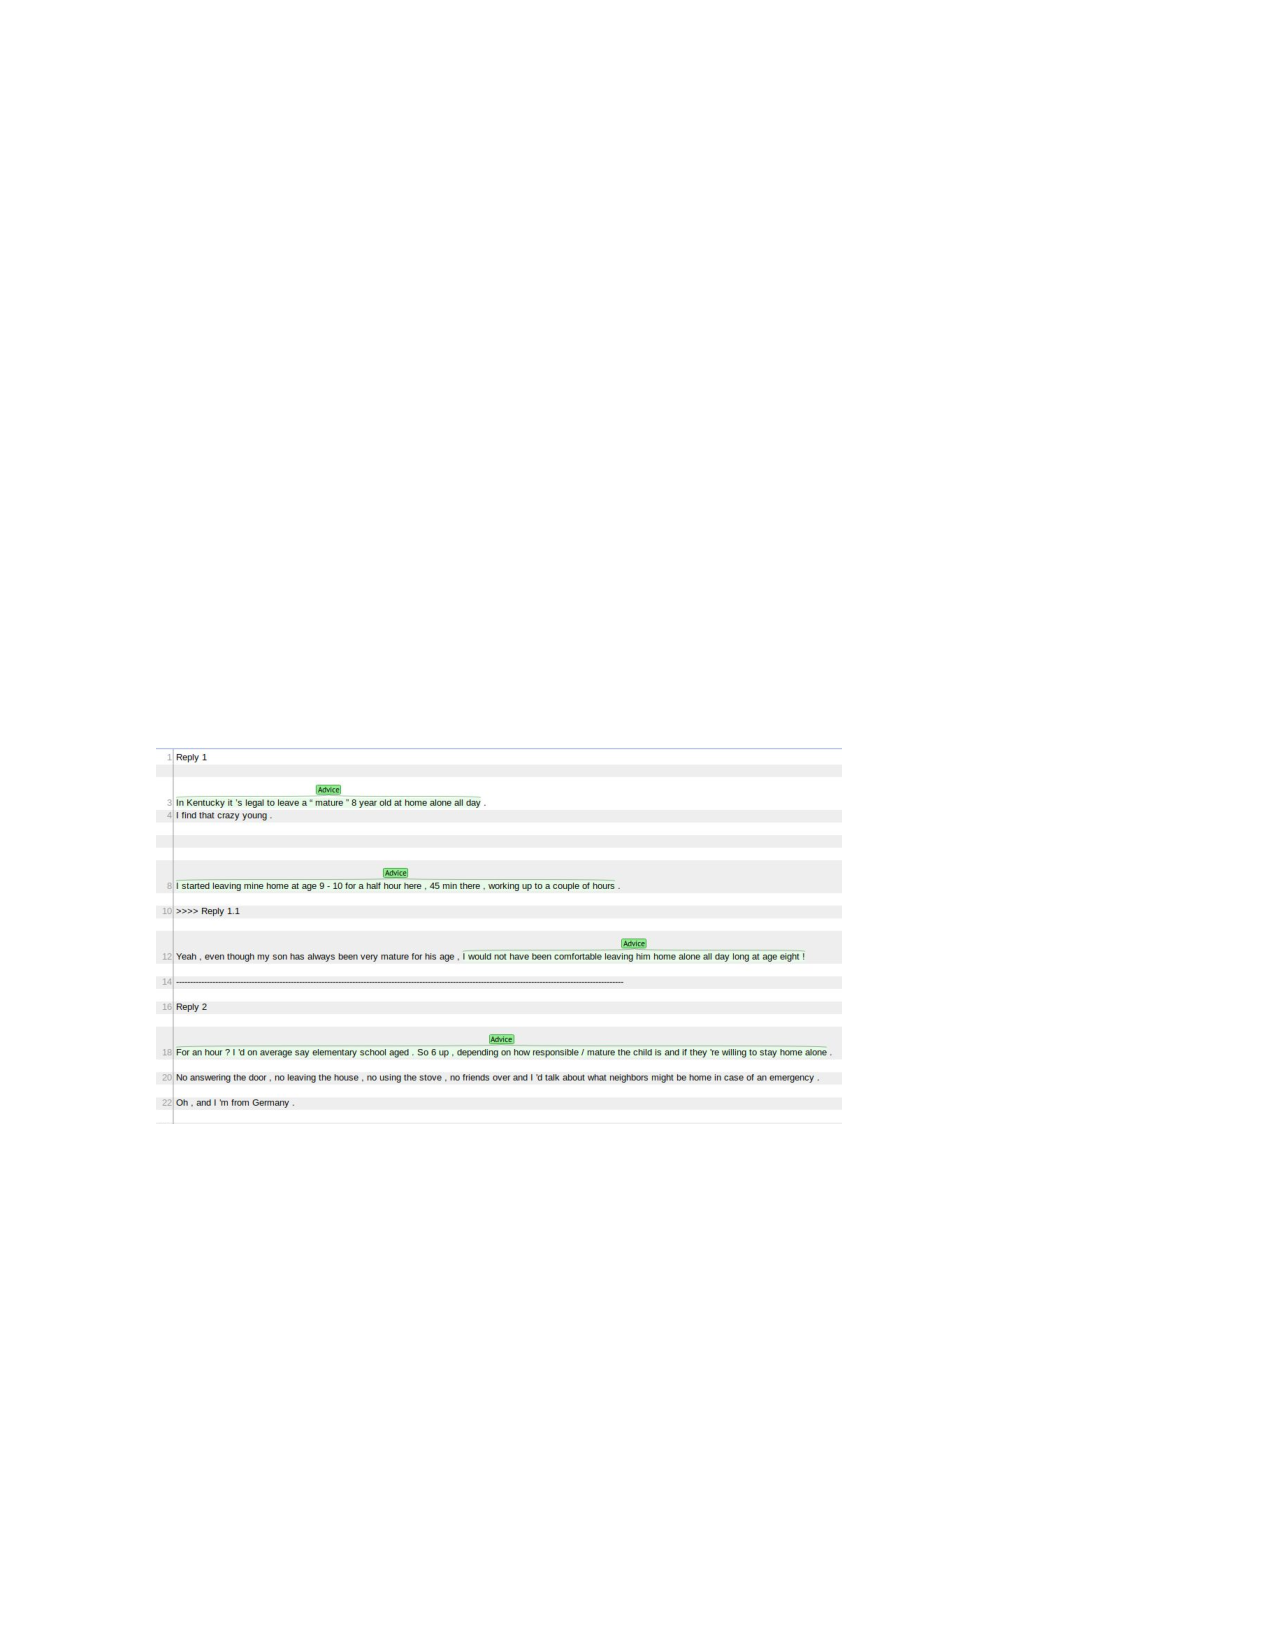
\includegraphics[width=\linewidth]{figures/ann-2.pdf}
        \caption{}
    \end{figure}

5 annotators on Amazon Mechanical Turk annotated each HIT of 5 comments.

\end{frame}


\begin{frame}[c]\frametitle{Label Aggregation}

We chose \textbf{sentences} as the units of advice.

How to aggregate sentence labels while accounting for inter-annotator variability?

\pause

\vfill

\begin{alertblock}{Dawid-Skene Labels}
        An EM based algorithm that estimates the label with the maximum estimated \textbf{posterior probability} by iteratively computing annotator competencies and type probabilities~\citep{dawid_maximum_1979}.
\end{alertblock}

\end{frame}


\begin{frame}[c]\frametitle{Dataset}
    \centering

    r/AskParents \quad 10,594 sentences \quad 407 posts

    r/needadvice \quad 7,862 sentences \quad 277 posts

    \vfill

    Data (and code) available at \href{https://github.com/venkatasg/Advice-EMNLP2020}{\sansc github.com/venkatasg/Advice-EMNLP2020}

\end{frame}


}

{
\metroset{sectionpage=none}
\section{Preliminary Analysis}
\begin{frame}[c]\frametitle{Advice Strategies}

\pause

\ex. \a.\label{ex:pers-1} I did the classic Ferberizing: check on baby after 5 mins,then 10 mins,then 20 mins, etc, until asleep. \only<3->{\alert{{\sansc personal narrative}}}\\
     \b.\label{ex:pers-2} Have you tried a calm spray? \only<4->{\alert{{\sansc questions}}}\\
     \b. \label{ex:pers-3} Figure out why they like them , and then recommend those ones\\for those reasons. \only<5->{\alert{{\sansc imperatives}}}\\
     \b. \label{ex:pers-4} If he doesn’t want therapy, maybe an antidepressant would \\help. \only<6->{\alert{{\sansc conditionals}}}\\

\vfill

\pause

\onslide<7->{To study personal narratives further, we (the authors) analyzed 213 sentences DS-labelled as advice for whether they contained personal narratives.}

\end{frame}

\begin{frame}[c]\frametitle{Personal Narratives}

\begin{figure}
\begin{tikzpicture}
   \begin{axis}[
       mbarplot,
       cycle list name=mbarplot cycle,
       width  = \columnwidth,
       height = 0.9\textheight,
       major x tick style = transparent,
       ybar=\pgflinewidth,
       bar width=15pt,
       ymajorgrids = true,
       ylabel style={rotate=-90, align=left},
       ylabel=\% of\\sents,
       symbolic x coords={r/AskParents, r/needadvice},
       xtick = data,
       tick label style={/pgf/number format/assume math mode=true},
       scaled y ticks = false,
       enlarge x limits=0.5,
       ymin=0,
       ymax=30,
       legend cell align=left,
       legend style={
               at={(0.95,1.03)},
               anchor=north,
               text=fgcolor,
               font=\small
       }
   ]
    \addplot+
           coordinates {(r/AskParents, 16.4) (r/needadvice, 6.33)};
   \end{axis}
\end{tikzpicture}
\caption{Y Axis shows \% of sentences that were judged to contain personal narratives.}
\end{figure}

\end{frame}


\begin{frame}[c]\frametitle{Non-advice}
    \pause
    \centering
    \begin{figure}
    \begin{tikzpicture}
    \pie[/tikz/nodes={text=white},text=inside, color={TolDarkPurple!70, TolDarkRed!70}]{32.3/Advice Sentences, 67.8/Non-Advice Sentences}
    \end{tikzpicture}
    \caption{Proportion of advice and non-advice in our dataset}
    \end{figure}
\end{frame}

\begin{frame}[c]\frametitle{Non-advice}

\ex. \a.\label{ex:nona-1}\textellipsis being fully prepared for an interview calmed me down \textellipsis \textbf<2->{ Good luck on your interviews and fingers crossed. } \only<2->{\alert{{\sansc sentiment}}}\\
     \b.\label{ex:nona-2}  Look for smaller outfits, they’re more likely to be willing to give you some time. \textbf<3->{Most professionals - if they have the time - are more than happy to talk to a student about what they do\textellipsis} \only<3->{\alert{{\sansc support}}}\\
     \b. \label{ex:nona-3} \textbf<4->{Yes, no one will ever know the big answers to the big questions.} What is the only thing that if shared , will grow larger in size? Answer: Love. Let that define your actions in life. \only<4->{\alert{{\sansc reasoning}}}\\

\end{frame}

\begin{frame}\frametitle{Lexical Analysis}

    \pause

    \begin{table}[t]
        \centering
        \small
        \begin{tabular}{lp{40mm}p{40mm}}
	\toprule
     & \textbf{Advice} & \textbf{Non-advice} \\
    \midrule
    {\multirow{8}{*}{\rotatebox{90}{\bfseries r/AskParents}}} & \hphantom{a} book if take something help then you might talk need down can etc play find show or great also give buy big watch diaper car about else minute spend baby & \hphantom{a} \textbf<3>{\alert<3>{luck}} \textbf<3>{\alert<3>{sorry}} \textbf<3>{\alert<3>{shit}} however dog crazy teenager op die eventually three wish weird daughter yeah brother example miss gender anyway anymore comment morning lol boyfriend girl younger \textbf<3>{\alert<3>{hope}} drive mine\\
    \midrule
    {\multirow{9}{*}{\rotatebox{90}{\bfseries r/needadvice}}}
    & \hphantom{a} he phone night adult stay set big game doctor fun bring less show love depend activity eat normal put teacher family etc minute teach allow home they area & \hphantom{a} \textbf<3>{\alert<3>{luck}} degree company college interview hobby student field mental course op \textbf<3>{\alert<3>{sorry}} job dog anxiety hire eventually position path \textbf<3>{\alert<3>{shit}} comment human online community shoe \textbf<3>{\alert<3>{thanks}} note exercise depression slowly\\
    \bottomrule
\end{tabular}

        \caption{Top 30 lemmas ranked by log-odds ratio}
        \label{tab:logodds}
    \end{table}
\end{frame}


}

{
\section{Modeling}
\begin{frame}[c]\frametitle{Models}

We model advice identification as a \textbf{binary classification task}.

\pause

\begin{description}[Language Modelling]\itemsep10pt
    \item[Rule-based] SEMEVAL 2019 baseline \& NTUA-IS 2019\citep{potamias-etal-2019-ntua}.

    Match and score against \alert{words}, \alert{phrases}, \alert{regexs}:\\ \textit{suggest}, \textit{recommend}, \textit{.*would\textbackslash slike.*if.*}

    \pause

    \item[Language Models] We use \alert{BERT} \citep{devlin_bert:_2019} and experiment with input:
    \begin{description}[Architectures]\itemsep10pt
        \item[BERT\textsubscript{sent\hphantom{qc}}] {\sansc [cls] sentence [sep]}
        \item[BERT\textsubscript{sent+q}] {\sansc [cls] sentence [sep] question}
        \item[BERT\textsubscript{sent+c}] {\sansc [cls] sentence [sep] context}
    \end{description}

\end{description}


\end{frame}


}

{
\metroset{sectionpage=none}
\section{Results}
\begin{frame}[c]\frametitle{Results}
\centering
\begin{figure}
    \begin{tikzpicture}
        \begin{axis}[
            mbarplot,
            cycle list name=mbarplot cycle,
            width  = \columnwidth,
            height = 0.9\textheight,
            major x tick style = transparent,
            ybar=\pgflinewidth,
            bar width=11pt,
            ymajorgrids = true,
            ylabel = {F1},
            ylabel style={rotate=-90},
            symbolic x coords={SEMEVAL, NTUA-IS, BERT\textsubscript{sent}, BERT\textsubscript{sent+c}, BERT\textsubscript{sent+q}},
            xtick = data,
            tick label style={/pgf/number format/assume math mode=true},
            scaled y ticks = false,
            enlarge x limits=0.2,
            ymin=0,
            ymax=100,
            legend cell align=left,
            legend style={
                    at={(0.9,0.99)},
                    anchor=north,
                    text=fgcolor,
                    font=\small
            }
        ]

        \addplot+[fill opacity=1,visible on=<2->, style={postaction={pattern=crosshatch dots}}]
                coordinates {(SEMEVAL, 57.2) (NTUA-IS, 53.5) (BERT\textsubscript{sent}, 77.8) (BERT\textsubscript{sent+c}, 77.6) (BERT\textsubscript{sent+q}, 72.5)};
        \addplot+[fill opacity=1,visible on=<3->]
                coordinates {(SEMEVAL, 44.6) (NTUA-IS, 42.3) (BERT\textsubscript{sent}, 51.9) (BERT\textsubscript{sent+c}, 51.9) (BERT\textsubscript{sent+q}, 37.4)};
        \legend{r/needadvice, r/AskParents}
        \end{axis}
    \end{tikzpicture}
    \caption{\onslide<2->{BERT\textsubscript{sent} has best performance.\\}\onslide<3->{Performance on r/AskParents worse than r/needadvice}}
\end{figure}
\end{frame}

}

{
\metroset{sectionpage=none}
\section{Analysis}
\begin{frame}[c]\frametitle{Performance on Personal Narratives}
\centering
\begin{figure}
\begin{tikzpicture}
   \begin{axis}[
       mbarplot,
       cycle list name=mbarplot cycle,
       width  = \columnwidth,
       height = 0.9\textheight,
       major x tick style = transparent,
       ybar=\pgflinewidth,
       bar width=15pt,
       ytick={0,20,...,100},
       tickwidth=0pt,
       ymajorgrids=true,
       ylabel = {F1},
       ylabel style={rotate=-90},
       symbolic x coords={AskParents, needadvice},
       xtick = data,
       tick label style={/pgf/number format/assume math mode=true},
       scaled y ticks = false,
       enlarge x limits=0.75,
       ymin=0,
       ymax=100,
       legend cell align=left,
       legend style={
               at={(0.9,0.99)},
               anchor=north,
               text=fgcolor,
               font=\small
       }
   ]
   \addplot+[fill opacity=1,visible on=<2->]
           coordinates {(AskParents, 51.9) (needadvice, 77.8)};
   \addplot+[fill opacity=1,visible on=<3->,style={postaction={pattern=crosshatch dots}}]
           coordinates {(AskParents, 32.2) (needadvice, 45.9)};

   \legend{{\sansc test set\hphantom{}}, {\sansc personal}}
   \end{axis}
\end{tikzpicture}
\caption{\onslide<3->{BERT\textsubscript{sent} performance on personal narrative sentences in test set suffers.}}
\end{figure}
\end{frame}
}

{
\metroset{sectionpage=none}
\section{Conclusion}
\begin{frame}[c]\frametitle{Conclusion}

\begin{description}[Advice Structures]\itemsep10pt
    \item[Dataset] We introduce a new dataset for \alert{advice given online}.

    \pause

    \item[Advice Structure] People use various \alert{strategies} when giving advice.

    \pause

    \item[Modeling] Language models learn some surface-level rules, but need to do better at \alert{implicit advice}.
\end{description}

\end{frame}
}

{
\metroset{numbering=none}
\section*{references}
\begin{frame}[allowframebreaks, noframenumbering]{References}
\printbibliography[heading=none]
\end{frame}
}

%Backup slides go here
\makeatletter
\renewcommand{\ExLBr}{\nfbc}
\renewcommand{\ExRBr}{\nfbc}
\makeatother

\appendix
\begin{frame}[standout]

{\huge \normalfont \sansc appendix}

\end{frame}

\begin{frame}[c]\frametitle{Gold Annotator Agreement}

\centering
\begin{tikzpicture}
  \begin{axis}[
      mbarplot,
      cycle list name=mbarplot cycle,
      width  = \columnwidth,
      height = 0.98\textheight,
      major x tick style = transparent,
      ybar=\pgflinewidth,
      bar width=15pt,
      ymajorgrids = true,
      ylabel = {Cohen's Kappa},
      symbolic x coords={r/AskParents, r/needadvice},
      xtick = data,
      tick label style={/pgf/number format/assume math mode=true},
      scaled y ticks = false,
      enlarge x limits=0.5,
      ymin=0,
      ymax=1,
      legend cell align=left,
      legend style={
              at={(0.9,0.99)},
              anchor=north,
              text=fgcolor,
             font=\normalsize
      }
  ]
   \addplot+
          coordinates {(r/AskParents, 0.620) (r/needadvice, 0.669)};
   \addplot+[style={postaction={pattern=crosshatch dots}}]
          coordinates {(r/AskParents, 0.680) (r/needadvice, 0.681)};
   \legend{$\kappa_{maj}$, $\kappa_{DS}$}
  \end{axis}
\end{tikzpicture}

\end{frame}

\begin{frame}[c]\frametitle{Average  Inter-Annotator Agreement}

\centering
\begin{tikzpicture}
  \begin{axis}[
      mbarplot,
      cycle list name=mbarplot cycle,
      width  = \columnwidth,
      height = 0.98\textheight,
      major x tick style = transparent,
      ybar=\pgflinewidth,
      bar width=15pt,
      ymajorgrids = true,
      ylabel = {Score},
      symbolic x coords={r/AskParents, r/needadvice},
      xtick = data,
      tick label style={/pgf/number format/assume math mode=true},
      scaled y ticks = false,
      enlarge x limits=0.5,
      ymin=0,
      ymax=100,
      legend cell align=left,
      legend style={
              at={(1.0,1.03)},
              anchor=north,
              text=fgcolor,
              font=\small
      }
  ]
  \addplot+
          coordinates {(r/AskParents, 83.71) (r/needadvice, 85.99)};
   \addplot+
          coordinates {(r/AskParents, 76.86) (r/needadvice, 85.71)};
   \addplot+
          coordinates {(r/AskParents, 79.62) (r/needadvice, 79.99)};
   \addplot+
          coordinates {(r/AskParents, 73.14) (r/needadvice, 79.55)};
   \legend{Accuracy, Precision, Recall, F1}
  \end{axis}
\end{tikzpicture}

\end{frame}

\begin{frame}[c]\frametitle{Lexical Analysis}

We quantify how strongly individual lemmas are associated with advice versus non-advice text using the log-odds ratio \citep{nye-nenkova-2015-identification}.

\vspace{5mm}

\begin{equation}
Odds(w,c) = \frac{P(w|c)}{1-P(w|c)}
\end{equation}

\begin{equation}
\text{log-odds ratio} = \frac{Odds(w,advice)}{Odds(w,non-advice))}
\end{equation}

\end{frame}

\begin{frame}[c]\frametitle{Generalizability Results}
\centering
\begin{tikzpicture}
  \begin{axis}[
      mbarplot,
      cycle list name=mbarplot cycle,
      width  = \columnwidth,
      height = 0.98\textheight,
      major x tick style = transparent,
      ybar=\pgflinewidth,
      bar width=15pt,
      ymajorgrids = true,
      ylabel = {F1},
      ylabel style={rotate=-90},
      symbolic x coords={r/AskParents, r/needadvice},
      xtick = data,
      tick label style={/pgf/number format/assume math mode=true},
      scaled y ticks = false,
      enlarge x limits=0.5,
      ymin=0,
      ymax=100,
      legend cell align=left,
      legend style={
              at={(0.9,0.99)},
              anchor=north,
              text=fgcolor,
              font=\small
      }
  ]
  \addplot+
          coordinates {(r/AskParents, 50.5) (r/needadvice, 77.8)};
   \addplot+[style={postaction={pattern=crosshatch dots}}]
          coordinates {(r/AskParents, 48.1) (r/needadvice, 76.0)};
   \legend{{\sansc normal\hphantom{er}}, {\sansc transfer}}
  \end{axis}
\end{tikzpicture}
\end{frame}

\begin{frame}[c]\frametitle{Dataset Metrics}
    \begin{table}[H]
        \centering
        \begin{tabular}{llll}
	\toprule
    \textbf{Dataset} & \textbf{Train} & \textbf{Dev} & \textbf{Test} \\
    \midrule
    AskParents & 8701(.29) & 802(.33) & 1091(.26)\\
    \midrule
    needadvice & 6148(.37) & 816(.34) & 898(.37) \\
    \bottomrule
\end{tabular}

        \caption{Sentence metrics in our dataset, with fraction DS-labeled as advice.}
        \label{tab:dataset-metrics}
    \end{table}
\end{frame}

\begin{frame}[c]\frametitle{Gold Internal Agreement}
    \begin{table}[H]
        \centering
        \begin{tabular}{llll}
	\toprule
    \textbf{Dataset} & \textbf{Sentences} & $\kappa_{maj}$ & $\kappa_{DS}$  \\
    \midrule
    AskParents & 203 & 0.620 & 0.669 \\
    \midrule
    needadvice & 110 & 0.680 & 0.681 \\
    \bottomrule
\end{tabular}

        \caption{Gold annotator agreement on the internal task.}
        \label{tab:internal-agreement}
    \end{table}
\end{frame}

\begin{frame}[c]\frametitle{Agreement}
    \begin{table}[H]
        \centering
        \begin{tabular}{lllll}
	\toprule
    \textbf{Dataset} & \textbf{Acc} & \textbf{P} & \textbf{R} & \textbf{F1}\\
    \midrule
    AskParents & 83.71 & 76.86 & 79.62 & 73.14 \\
    \midrule
    needadvice & 85.99 & 85.71 & 79.99 & 79.55 \\
    \bottomrule
\end{tabular}


        \caption{Average inter-annotator agreement for all workers against DS labels}
        \label{tab:agreement}
    \end{table}
\end{frame}

\begin{frame}[c]\frametitle{Discourse Modes}
    \begin{table}[H]
        \centering
        \begin{tabular}{lll}
	\toprule
    \textbf{Subreddit} & \textbf{Other (\%)} & \textbf{Personal}\\
     &  & \textbf{Narrative (\%)}\\
    \midrule
    \textbf{r/AskParents} & 83.6 & 16.4\\
    \midrule
    \textbf{r/needadvice} & 93.67 & 6.33 \\
    \textbf{\quad-Career} & 100 & 0\\
    \textbf{\quad-Mental Health} & 81.82 & 18.18\\
    \textbf{\quad-Friendships} & 100 & 0\\
    \textbf{\quad-Education} & 95.4 & 4.6\\
    \textbf{\quad-Life Decisions} & 88.9 & 11.1\\
    \bottomrule
\end{tabular}

        \caption{Modes of discourse for advice sentences in each flair/subreddit}
        \label{tab:disc-modes}
    \end{table}
\end{frame}

\begin{frame}[c]\frametitle{Results-Classification}
    \begin{table}[H]
        \centering
        \begin{tabular}{cllll}
	\toprule
    & \textbf{Model} & \textbf{P} & \textbf{R} & \textbf{F1} \\
    \midrule
    {\multirow{6}{*}{\rotatebox{90}{\tiny r/AskParents}}} & SEMEVAL & 32.7 & 70.2 & 44.6 \\
    & NTUA-IS & 31.4 & 64.9 & 42.3 \\
    & BERT$_{\text{noft}}$ & 62.6 (1.2) & 14.9 (1.0) & 24.0 (1.4) \\
    & BERT$_{\text{sent}}$ & 54.9 (2.4) & 49.5 (4.4) & \textbf{51.9} (1.9) \\
    & BERT$_{\text{sent+c}}$ & 54.2 (2.1) & 49.9 (4.0) & 51.9 (2.2) \\
    & BERT$_{\text{sent+q}}$ & 61.0 (13.4) & 33.1 (11.9) & 37.4 (8.1) \\
   \midrule
   {\multirow{6}{*}{\rotatebox{90}{\tiny r/needadvice}}} & SEMEVAL & 44.5 & 80.3 & 57.2 \\
    & NTUA-IS & 43.0 & 70.9 & 53.5 \\
    & BERT$_{\text{noft}}$ & 82.9 (0.5) & 44.6 (1.4) & 58.0 (1.2) \\
    & BERT$_{\text{sent}}$ & 79.7 (3.8) & 76.3 (3.9) & \textbf{77.8} (0.3) \\
    & BERT$_{\text{sent+c}}$ & 80.4 (4.4) & 75.3 (4.4) & 77.6 (0.7) \\
    & BERT$_{\text{sent+q}}$ & 83.4 (4.8) & 64.7 (7.4) & 72.5 (3.5) \\
    \bottomrule
\end{tabular}
        \caption{Classification results on test set.}
        \label{tab:results-class}
    \end{table}
\end{frame}

\begin{frame}[c]\frametitle{Results-Generalization}
    \begin{table}[H]
        \centering
        \begin{tabular}{lccc}
	\toprule
    \textbf{Model} & \textbf{P} & \textbf{R} & \textbf{F1} \\
    \midrule
     AP $\to$ AP & 54.9 (2.4) & 49.5 (4.4) & 51.9 (1.9) \\
     AP$_{p}$ $\to$ AP & 59.1 (3.5) & 44.4 (4.1) & 50.5 (1.8) \\
     NA $\to$ AP & 61.9 (4.9) & 39.7 (3.5) & 48.1 (1.3) \\
    \midrule
     NA $\to$ NA & 79.7 (3.8) & 76.3 (3.9) & 77.8 (0.3) \\
     AP $\to$ NA & 74.0 (4.0) & 79.3 (2.9) & 76.5 (0.9) \\
     AP$_{p}$ $\to$ NA & 76.9 (3.8) & 75.5 (4.7) & 76.0 (1.1) \\
    \bottomrule
\end{tabular}
        \caption{Generalizbility results on test set.}
        \label{tab:results-gen}
    \end{table}
\end{frame}

\begin{frame}[c]\frametitle{Results-Flair}
    \begin{table}[H]
        \centering
        \begin{tabular}{llll}
	\toprule
    \textbf{Flair} & \textbf{P} & \textbf{R} & \textbf{F1} \\
    \midrule
    Friendships & 85.5 (5.7) & 93.8 (0.0) & 89.2 (2.9) \\
    Mental Health & 75.6 (3.5) & 74.7 (3.6) & 75.0 (0.6) \\
    Education & 86.8 (2.9) & 67.4 (6.2) & 75.7 (3.1) \\
    Career & 75.9 (5.1) & 78.0 (3.8) & 76.7 (1.3)\\
    Life Decisions & 82.4 (4.4) & 82.8 (3.5) & 82.4 (0.7) \\
    \bottomrule
\end{tabular}
        \caption{Flair results on test set.}
        \label{tab:results-flair}
    \end{table}
\end{frame}

\begin{frame}[c]\frametitle{Attention}
   \begin{figure}
       \centering
       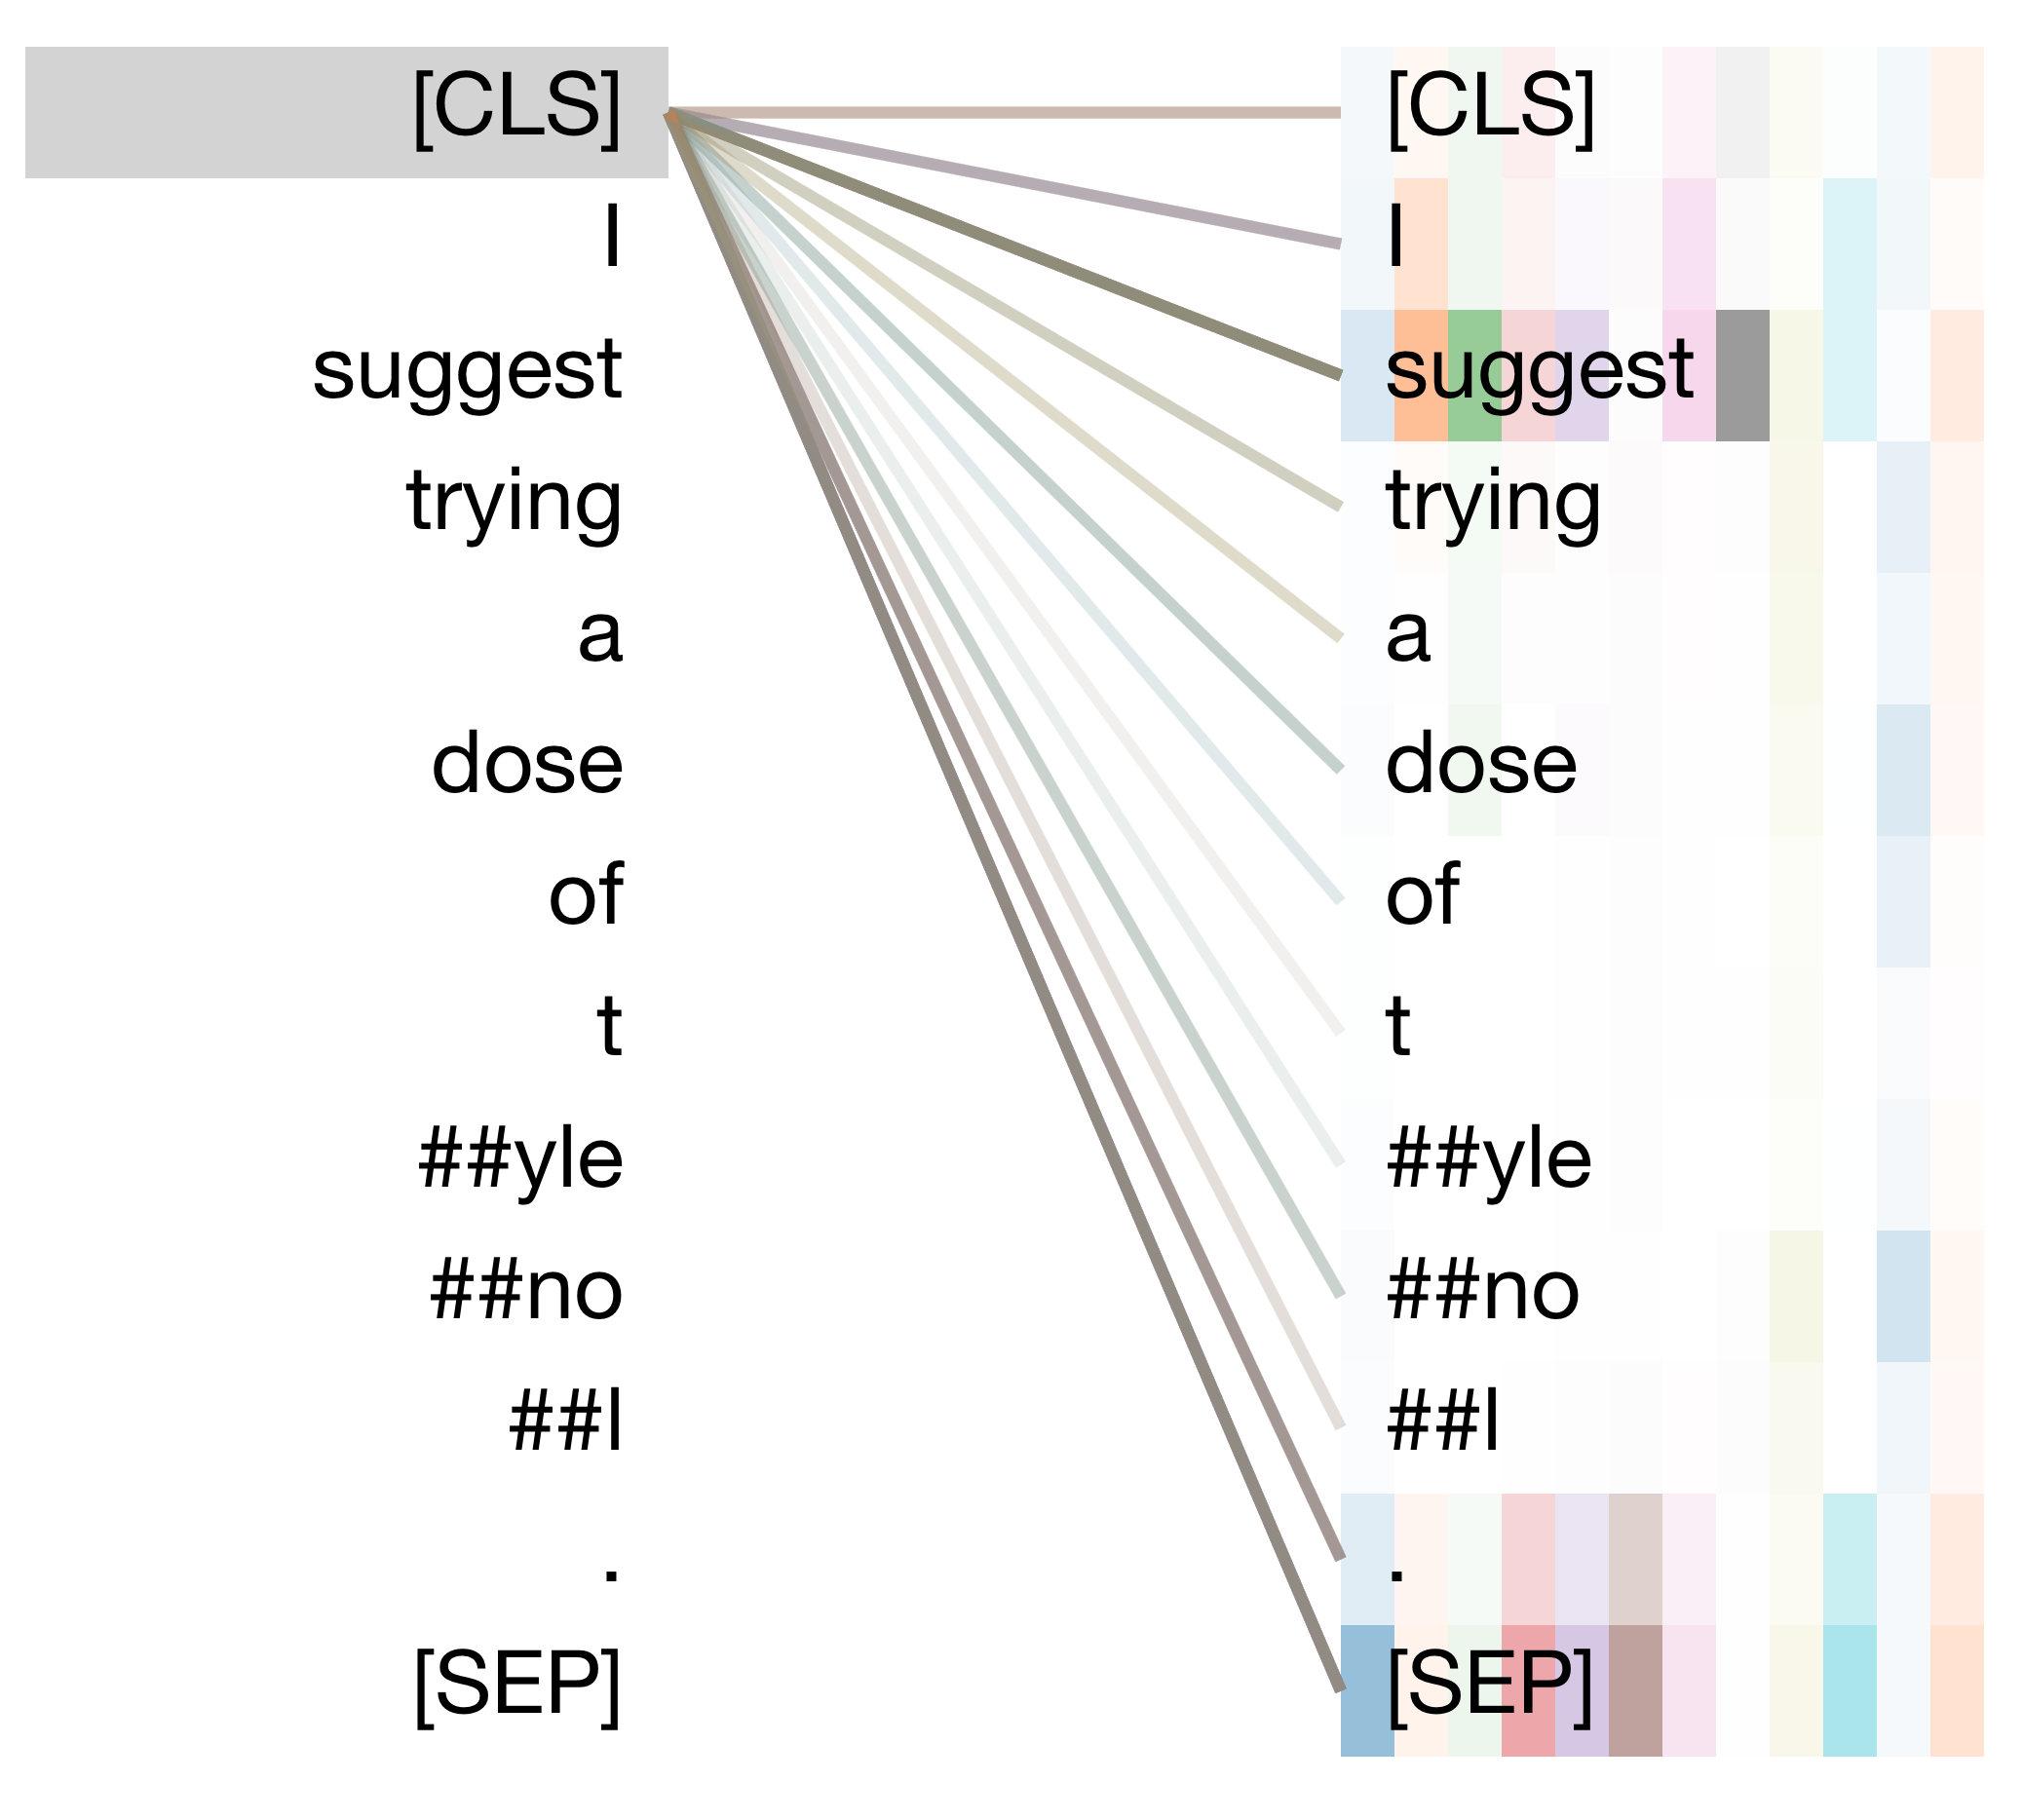
\includegraphics[width=0.75\linewidth]{figures/att-2.png}
       \caption{Attention weights visualized using BertViz~\citep{vig2019transformervis}}
   \end{figure}
\end{frame}

\begin{frame}[c]\frametitle{Attention}
    \begin{figure}
        \centering
        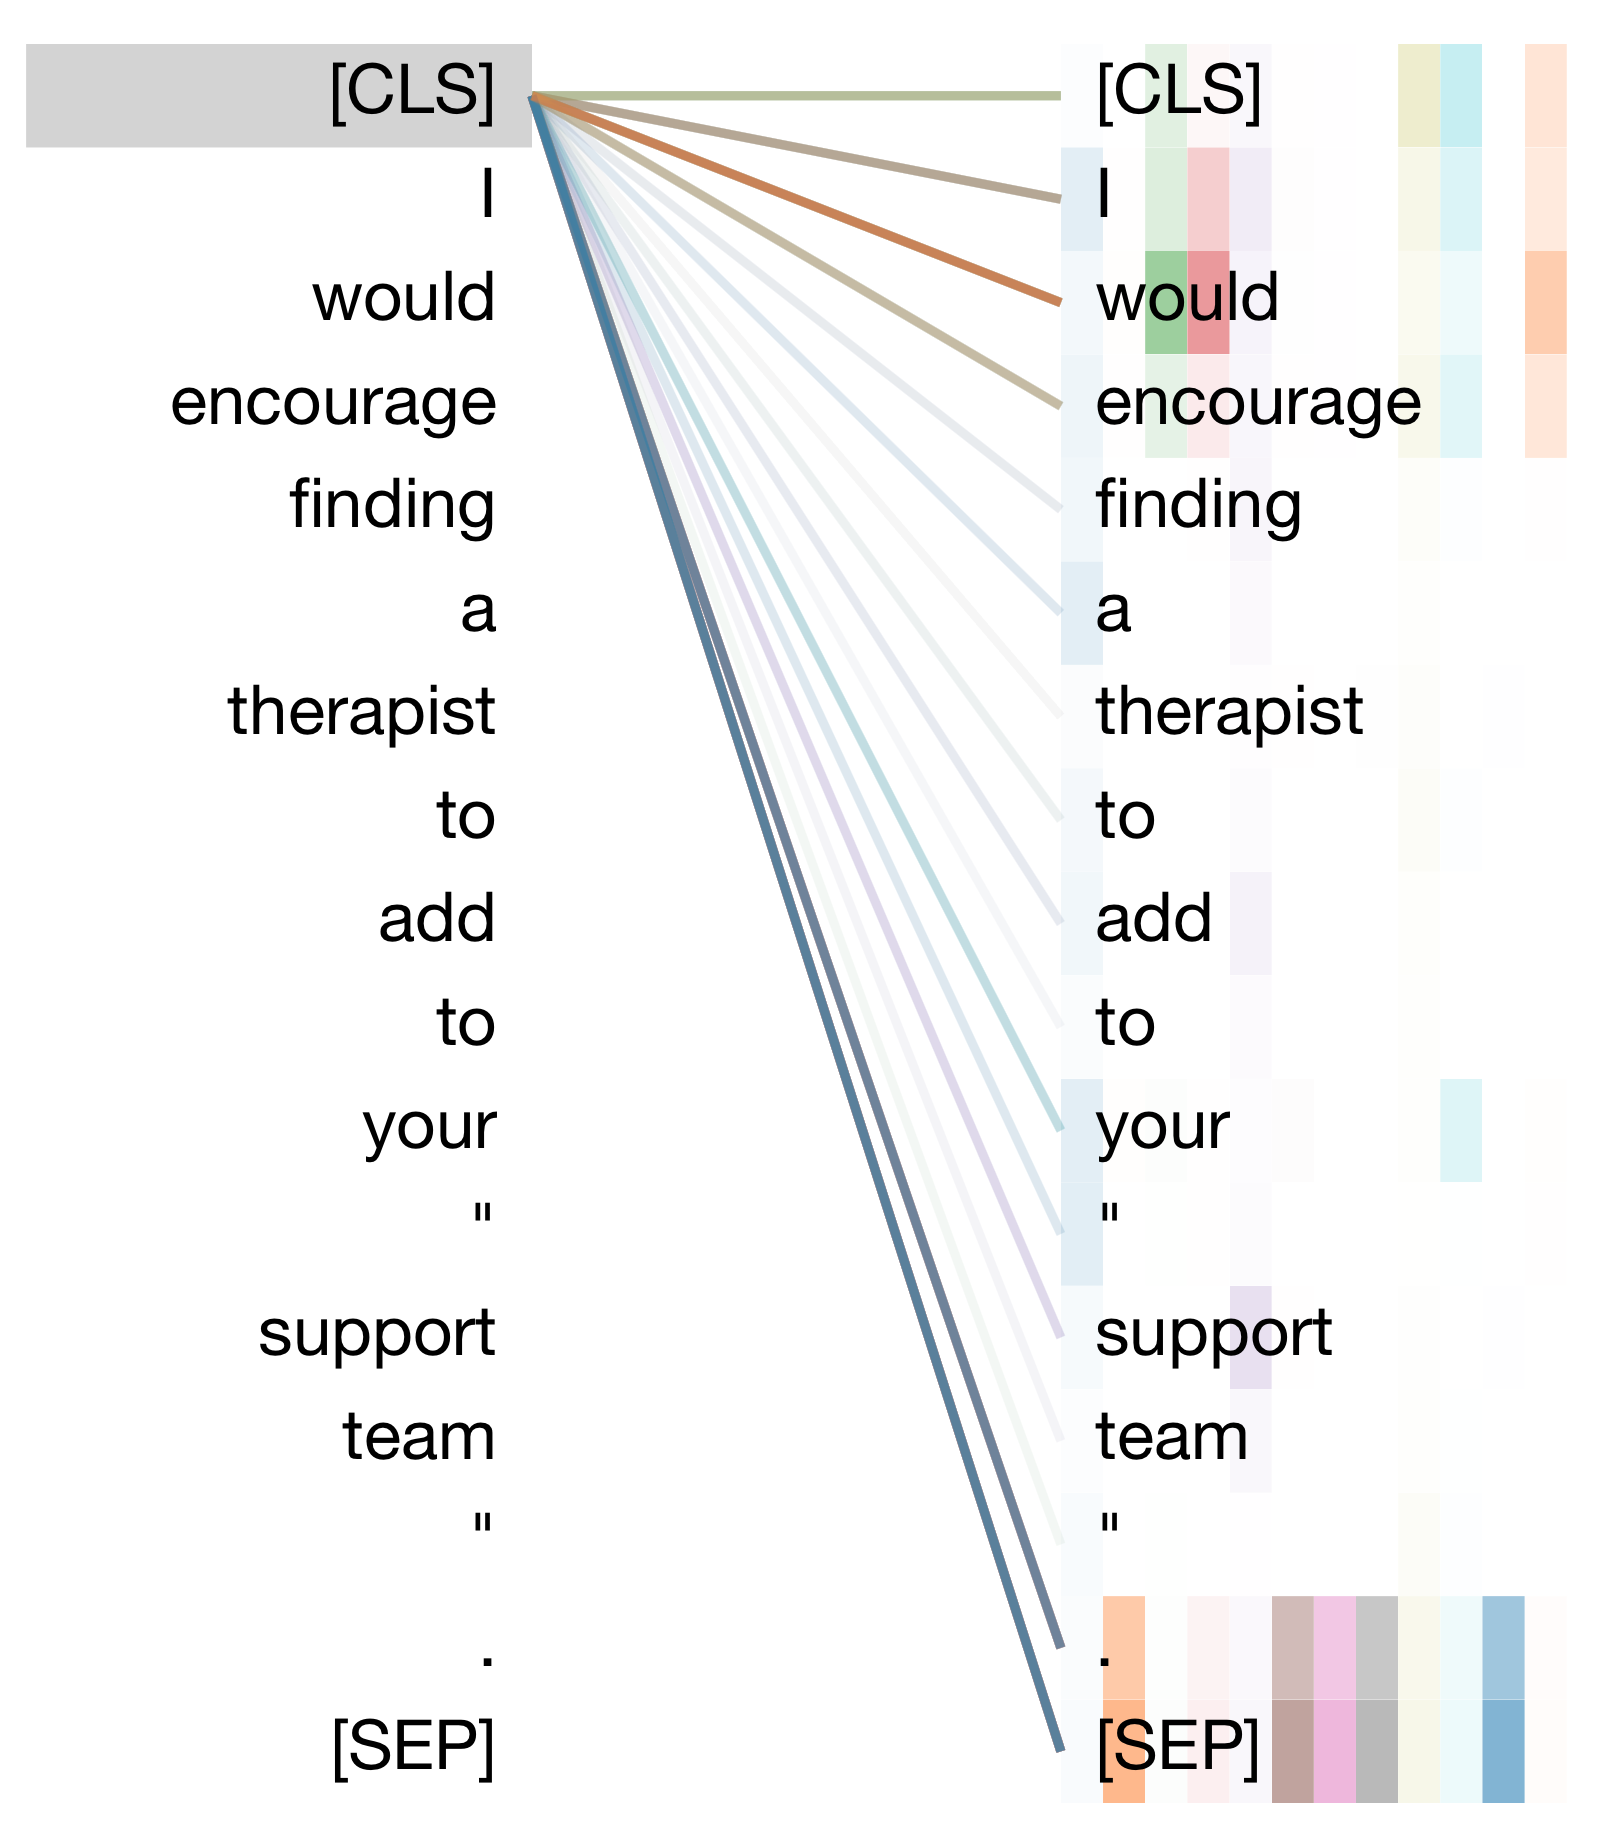
\includegraphics[width=0.6\linewidth]{figures/att-1.png}
        \caption{Attention weights visualized using BertViz~\citep{vig2019transformervis}}
    \end{figure}
\end{frame}


\end{document}
